\begin{frameExample}{Mezcla de Productos (Fracciones)}{}
  % EXAMPLE 2.6-7 (Product Mix Problem) Gupta
Una empresa fabrica tres productos A, B y C. El tiempo para fabricar el producto A es el doble que para B y tres veces para C y si toda la mano de obra se dedica a la fabricación del producto A, se pueden producir 1,600 unidades de este producto. Estos productos deben producirse en una proporción de 3: 4: 5. Hay demanda de al menos 300, 250 y 200 unidades de productos A, B y C y el beneficio obtenido por unidad es de \$ 90, \$ 40 y \$ 30 respectivamente. Formule el problema como un problema de programación lineal.

{\centering
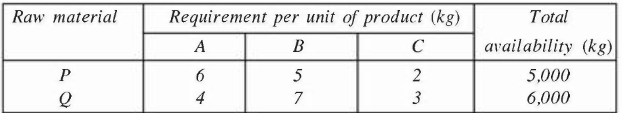
\includegraphics[scale=0.5]{example_product-mix02_gupta}
\par}

\end{frameExample}

\begin{frameExample}{Mezcla de Productos (Fracciones)}{}
  \begin{columns}[t]
    \column{0.5\textwidth}
      \begin{flalign*}
    \max Z = 90x_1 + 40x_2 + 30x_3 & \\
    \intertext{Subject to (s.t.)}
    6x_1 + 5x_2 + 2x_3 & \leq 5000\\
    4x_1 + 7x_2 + 3x_3 & \leq 6000\\
    x_1 + \frac{x_2}{2} + \frac{x_3}{3} & \leq 1600
  \end{flalign*}
  \column{0.5\textwidth}
  \begin{flalign*}
        x_1 & \geq 300 \\
    x_2 & \geq 250\\
    x_3 & \geq 200\\[4mm]
    \frac{x_1}{3} &= \frac{x_2}{4}\\
    \frac{x_2}{4} & = \frac{x_3}{5}\\[4mm]
    x_1, x_2, x_3 &\geq 0
  \end{flalign*}
  \end{columns}
\end{frameExample}

%%% Local Variables:
%%% mode: latex
%%% TeX-master: "../slides"
%%% End:
